\section{2-kategorie i bikategorie}\label{cat:sec:two-categories}

W teorii kategorii zwykłych rozróżniamy obiekty i morfizmy. Funktory i transformacje naturalne pokazują, że warto rozważać również morfizmy pomiędzy morfizmami. Wprowadzimy najpierw 2-kategorie ścisłe, w których składanie 1-morfizmów jest ściśle łączne, a następnie osłabimy ten warunek do odpowiednio zgodnych izomorfizmów. Korzystamy z rozdziałów~\ref{sec:naturalne}, \ref{cat:sec:monoidal}, \ref{cat:sec:coherence} oraz \ref{cat:sec:enriched}.

\subsection{2-kategorie ścisłe}

\begin{definicja}[2-kategoria ścisła]\label{cat:def:strict-two-category}
2-kategoria ścisła $\mathcal K$ składa się z następujących danych:
\begin{enumerate}
\item klasy obiektów;
\item kategorii $\mathcal K(A,B)$ dla każdej pary obiektów $A,B$;
\item funktorów składania
\[
 M_{A,B,C}:\mathcal K(B,C)\times\mathcal K(A,B)
 \longrightarrow\mathcal K(A,C);
\]
\item wybranego obiektu $1_A\in\Ob(\mathcal K(A,A))$ dla każdego $A$.
\end{enumerate}
Obiekty kategorii $\mathcal K(A,B)$ nazywamy 1-morfizmami $A\to B$, a jej morfizmy $f\Rightarrow g$ nazywamy 2-morfizmami. Składanie w kategorii $\mathcal K(A,B)$ nazywamy pionowym i zapisujemy $\beta\circ\alpha$. Działanie $M$ na obiektach zapisujemy $gf$, a na morfizmach $\beta\ast\alpha$ i nazywamy składaniem poziomym.

Wymagamy ścisłej łączności składania poziomego oraz ścisłych praw jednostki zarówno na 1-morfizmach, jak i na 2-morfizmach:
\[
\begin{aligned}
 h(gf)&=(hg)f,&
 \gamma\ast(\beta\ast\alpha)&=(\gamma\ast\beta)\ast\alpha,\\
 1_B f&=f=f1_A,&
 \id_{1_B}\ast\alpha&=\alpha=\alpha\ast\id_{1_A}.
\end{aligned}
\]
W ostatnim równaniu $\alpha:f\Rightarrow g$ dla $f,g:A\to B$. Kategorię $\mathcal K(A,B)$ nazywamy kategorią morfizmów.
\end{definicja}

Przyjmujemy, że kategorie morfizmów są lokalnie małe. Jeżeli ich klasy obiektów są zbiorami, mówimy, że kategorie morfizmów są małe. Rozróżnienie jest istotne przy rozważaniu kategorii wszystkich kategorii.

\begin{center}
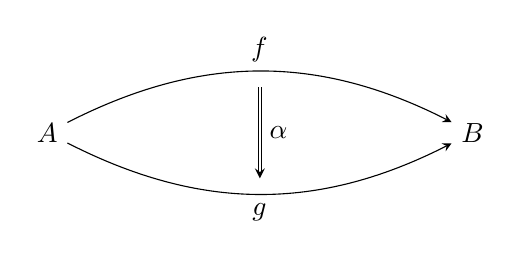
\begin{tikzpicture}[>=stealth]
 \node (a) at (0,0) {$A$};
 \node (b) at (5.4,0) {$B$};
 \draw[->] (a) to[bend left=27] node[above] {$f$} (b);
 \draw[->] (a) to[bend right=27] node[below] {$g$} (b);
 \draw[double,->] (2.7,.58)--node[right] {$\alpha$}(2.7,-.58);
\end{tikzpicture}
\end{center}
Strzałka podwójna oznacza 2-morfizm pomiędzy równoległymi 1-morfizmami, a nie dodatkowy 1-morfizm $A\to B$.

\begin{stwierdzenie}[Prawo wymiany]\label{cat:prop:two-interchange}
Dla 2-morfizmów
\[
 \alpha:f_0\Rightarrow f_1,\quad \alpha':f_1\Rightarrow f_2,
 \qquad
 \beta:g_0\Rightarrow g_1,\quad \beta':g_1\Rightarrow g_2,
\]
gdzie $f_i:A\to B$, $g_i:B\to C$, zachodzi
\[
 (\beta'\circ\beta)\ast(\alpha'\circ\alpha)
 =(\beta'\ast\alpha')\circ(\beta\ast\alpha).
\]
Ponadto $\id_g\ast\id_f=\id_{gf}$.
\end{stwierdzenie}
\begin{proof}
W kategorii iloczynu $\mathcal K(B,C)\times\mathcal K(A,B)$ mamy
\[
 (\beta',\alpha')\circ(\beta,\alpha)
 =(\beta'\circ\beta,\alpha'\circ\alpha).
\]
Stosując funktor $M_{A,B,C}$ i korzystając z zachowywania składania, otrzymujemy pierwszą równość. Morfizm $(\id_g,\id_f)$ jest identycznością obiektu $(g,f)$ w kategorii iloczynu; zachowywanie identyczności przez $M$ daje drugą równość.
\end{proof}

Pionowe i poziome składanie można przedstawić na jednym diagramie. Każdy wiersz odpowiada parze składanych 1-morfizmów, a każda kolumna pionowemu składaniu 2-morfizmów:
\begin{center}
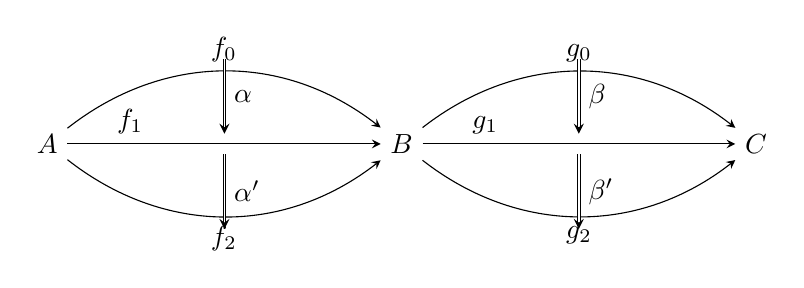
\begin{tikzpicture}[>=stealth]
 \node (a) at (0,0) {$A$};
 \node (b) at (4.5,0) {$B$};
 \node (c) at (9,0) {$C$};
 \draw[->] (a) to[bend left=38] node[above] {$f_0$} (b);
 \draw[->] (a)--node[above,pos=.2] {$f_1$}(b);
 \draw[->] (a) to[bend right=38] node[below] {$f_2$} (b);
 \draw[->] (b) to[bend left=38] node[above] {$g_0$} (c);
 \draw[->] (b)--node[above,pos=.2] {$g_1$}(c);
 \draw[->] (b) to[bend right=38] node[below] {$g_2$} (c);
 \draw[double,->] (2.25,1.08)--node[right] {$\alpha$}(2.25,.13);
 \draw[double,->] (2.25,-.13)--node[right] {$\alpha'$}(2.25,-1.08);
 \draw[double,->] (6.75,1.08)--node[right] {$\beta$}(6.75,.13);
 \draw[double,->] (6.75,-.13)--node[right] {$\beta'$}(6.75,-1.08);
\end{tikzpicture}
\end{center}
Prawo wymiany oznacza, że najpierw możemy złożyć pionowo obie kolumny, a potem poziomo, albo najpierw poziomo oba piętra, a potem pionowo. Wynik w obu przypadkach jest 2-morfizmem $g_0f_0\Rightarrow g_2f_2$.

\begin{stwierdzenie}[Równoważny opis aksjomatów]\label{cat:prop:two-axioms-equivalence}
W definicji~\ref{cat:def:strict-two-category} można zastąpić funktory $M$ działaniami na obiektach i morfizmach, wymagając odpowiednich typów, prawa wymiany oraz $\id_g\ast\id_f=\id_{gf}$. Pozostałe warunki pozostają bez zmian.
\end{stwierdzenie}
\begin{proof}
Dla każdej pary obiektów $(g,f)$ kategorii iloczynu definiujemy $M(g,f)=gf$. Morfizm $(\beta,\alpha):(g,f)\to(g',f')$ ma obraz $\beta\ast\alpha:gf\Rightarrow g'f'$. Prawo wymiany daje dokładnie zachowywanie składania każdej pary składanych morfizmów w iloczynie, a równość dla identyczności daje zachowywanie identyczności. Są to wszystkie aksjomaty funktora. Implikacja odwrotna jest treścią stwierdzenia~\ref{cat:prop:two-interchange}.
\end{proof}

\subsection{Składanie z 1-morfizmami}

Dla $\alpha:f\Rightarrow g$ w $\mathcal K(A,B)$ oraz $h:B\to C$, $k:D\to A$ definiujemy składanie z 1-morfizmami (ang.\ \emph{whiskering})
\[
 h\alpha=\id_h\ast\alpha:hf\Rightarrow hg,\qquad
 \alpha k=\alpha\ast\id_k:fk\Rightarrow gk.
\]

\begin{stwierdzenie}\label{cat:prop:two-whiskering}
Składanie z ustalonym 1-morfizmem definiuje funktory pomiędzy odpowiednimi kategoriami morfizmów. Dla $\alpha:f\Rightarrow f'$ oraz $\beta:g\Rightarrow g'$ przy $f,f':A\to B$, $g,g':B\to C$ zachodzi
\[
 \beta\ast\alpha=(\beta f')\circ(g\alpha)
 =(g'\alpha)\circ(\beta f).
\]
\end{stwierdzenie}
\begin{proof}
Dla ustalonego $h$ i pionowo składanych $\alpha,\alpha'$ prawo wymiany daje
\[
 h(\alpha'\circ\alpha)
 =(\id_h\circ\id_h)\ast(\alpha'\circ\alpha)
 =(h\alpha')\circ(h\alpha).
\]
Ponadto $h\id_f=\id_h\ast\id_f=\id_{hf}$. Zatem składanie z $h$ z lewej strony jest funktorem. Dla ustalonego $k$ analogiczny rachunek ma postać
\[
 (\alpha'\circ\alpha)k
 =(\alpha'\circ\alpha)\ast(\id_k\circ\id_k)
 =(\alpha' k)\circ(\alpha k),\qquad
 \id_f k=\id_{fk}.
\]
W kategorii iloczynu morfizm $(\beta,\alpha)$ można przedstawić na dwa sposoby:
\[
 (\beta,\id_{f'})\circ(\id_g,\alpha)
 =(\beta,\alpha)
 =(\id_{g'},\alpha)\circ(\beta,\id_f).
\]
Stosując funktor składania $M$, dostajemy żądaną równość.
\end{proof}

\begin{center}
\begin{tikzpicture}[>=stealth]
 \node (a) at (0,2.7) {$gf$};
 \node (b) at (5.2,2.7) {$gf'$};
 \node (c) at (0,0) {$g'f$};
 \node (d) at (5.2,0) {$g'f'$};
 \draw[->] (a)--node[above] {$g\alpha$}(b);
 \draw[->] (a)--node[left] {$\beta f$}(c);
 \draw[->] (b)--node[right] {$\beta f'$}(d);
 \draw[->] (c)--node[below] {$g'\alpha$}(d);
\end{tikzpicture}
\end{center}
Jest to kwadrat przemienny w zwykłej kategorii $\mathcal K(A,C)$: jego wierzchołkami są 1-morfizmy, a krawędziami 2-morfizmy.

\subsection{Przykłady 2-kategorii}

\begin{przyklad}[2-kategoria małych kategorii]\label{cat:ex:two-cat}
Niech $\mathbf{Cat}$ ma jako obiekty małe kategorie, jako 1-morfizmy funktory, a jako 2-morfizmy transformacje naturalne. Kategorie morfizmów to kategorie funktorów z pionowym składaniem ze stwierdzenia~\ref{cat:prop:vertical}. Składanie poziome jest dane wzorem z definicji~\ref{cat:def:horizontal}. Jego naturalność wykazano w stwierdzeniu~\ref{cat:prop:horizontal}, a prawo wymiany w twierdzeniu~\ref{cat:thm:interchange}. Identyczności spełniają $\id_G\ast\id_F=\id_{GF}$, ponieważ w każdym obiekcie $X$ lewa strona ma składową $\id_{GF(X)}$. Otrzymujemy funktory $M$ przez stwierdzenie~\ref{cat:prop:two-axioms-equivalence}. Ścisła łączność na 1-morfizmach wynika z łączności składania funktorów, a na 2-morfizmach ze stwierdzenia~\ref{cat:prop:horizontal-assoc}, które daje również prawa jednostki. Zatem $\mathbf{Cat}$ jest 2-kategorią ścisłą.

Dla małych kategorii $\mathcal A,\mathcal B$ zbiór funktorów jest podzbiorem iloczynu zbiorów odwzorowań na obiektach i morfizmach. Rodziny transformacji naturalnych są także indeksowane zbiorem obiektów. Wobec tego kategorie morfizmów $\mathbf{Cat}(\mathcal A,\mathcal B)$ są małe.
\end{przyklad}

\begin{przyklad}[Kategorie lokalnie dyskretne i lokalnie uporządkowane]\label{cat:ex:two-locally-discrete}
Każdą lokalnie małą kategorię zwykłą $\mathcal C$ można traktować jako 2-kategorię ścisłą, biorąc dla $\mathcal K(A,B)$ kategorię dyskretną na zbiorze $\Hom_{\mathcal C}(A,B)$. Jedynymi 2-morfizmami są identyczności. Składanie $\mathcal C$ na obiektach jednoznacznie wyznacza funktory składania między kategoriami dyskretnymi. Wszystkie aksjomaty redukują się do aksjomatów $\mathcal C$.

Inny przykład otrzymujemy z częściowo uporządkowanych zbiorów i odwzorowań monotonicznych. W kategorii morfizmów przyjmujemy punktowy porządek $f\leq g$ wtedy i tylko wtedy, gdy $f(x)\leq g(x)$ dla każdego $x$. Istnieje jeden 2-morfizm $f\Rightarrow g$ dokładnie wtedy, gdy $f\leq g$. Jeżeli $f\leq f'$ oraz $g\leq g'$, to dla każdego $x$ mamy
\[
 g(f(x))\leq g(f'(x))\leq g'(f'(x)).
\]
Pierwsza nierówność wynika z monotoniczności $g$, druga z porządku punktowego. Składanie jest więc monotoniczne na parach, a zatem jest funktorem kategorii uporządkowanych. Ścisłe aksjomaty na 1-morfizmach wynikają ze składania funkcji, a na 2-morfizmach z jednoznaczności morfizmów między ustaloną parą obiektów kategorii uporządkowanej.
\end{przyklad}

\begin{przyklad}[Jednoobiektowe 2-kategorie]\label{cat:ex:two-one-object}
Ścisła kategoria monoidalna $(\mathcal M,\otimes,I)$ wyznacza 2-kategorię ścisłą o jednym obiekcie $*$, z kategorią morfizmów $\mathcal K(*,*)=\mathcal M$, funktorem składania $\otimes$ i 1-morfizmem identycznościowym $I$. Przy konwencji $gf=g\otimes f$ ścisła łączność i jednostkowość wynikają dokładnie ze ścisłości struktury monoidalnej. Odwrotnie, jedyna kategoria morfizmów jednoobiektowej 2-kategorii ścisłej jest kategorią monoidalną z takim iloczynem i jednostką. Nie wymagamy symetrii struktury monoidalnej.
\end{przyklad}

\begin{uwaga}
W sensie definicji~\ref{cat:def:enriched-category} 2-kategorie ścisłe o małych kategoriach morfizmów są kategoriami wzbogaconymi w zwykłej kategorii małych kategorii z iloczynem kartezjańskim. Izomorfizmy łączności i jednostek iloczynu kartezjańskiego zmieniają wyłącznie nawiasowanie krotek. Po odczytaniu aksjomatów wzbogacenia na obiektach i morfizmach kategorii dostajemy dokładnie ścisłe równania składania poziomego; odwrotnie te równania zapewniają równość funktorów w aksjomatach wzbogacenia. Przy dużych kategoriach morfizmów należy odpowiednio powiększyć kategorię bazową lub przyjąć stosowne uniwersum.
\end{uwaga}

\subsection{Argument Eckmanna--Hiltona}

\begin{twierdzenie}[Argument Eckmanna--Hiltona]\label{cat:thm:eckmann-hilton}
Niech zbiór $S$ będzie wyposażony w dwie operacje monoidalne $\circ,\ast$ o wspólnej jednostce $e$, spełniające
\[
 (a\circ b)\ast(c\circ d)=(a\ast c)\circ(b\ast d).
\]
Wówczas obie operacje są równe i przemienne.
\end{twierdzenie}
\begin{proof}
Dla $x,y\in S$ z prawa wymiany i praw jednostki wynika
\[
 x\ast y=(x\circ e)\ast(e\circ y)
 =(x\ast e)\circ(e\ast y)=x\circ y.
\]
Jednocześnie
\[
 x\ast y=(e\circ x)\ast(y\circ e)
 =(e\ast y)\circ(x\ast e)=y\circ x.
\]
Stąd $x\circ y=y\circ x$ i $\ast=\circ$.
\end{proof}

\begin{wniosek}\label{cat:cor:two-unit-endomorphism}
Dla obiektu $A$ w 2-kategorii ścisłej endomorfizmy 1-morfizmu identycznościowego,
\[
 S=\Hom_{\mathcal K(A,A)}(1_A,1_A),
\]
tworzą monoid przemienny. Składanie pionowe i poziome na $S$ są równe. Odwracalne 2-morfizmy tworzą grupę abelową.
\end{wniosek}
\begin{proof}
Składanie pionowe ma jednostkę $\id_{1_A}$. Ponieważ $1_A1_A=1_A$, składanie poziome jest również operacją na $S$ i ma tę samą jednostkę przez ścisłe prawa jednostki 2-kategorii. Łączność obu operacji wynika z aksjomatów, a prawo wymiany ze stwierdzenia~\ref{cat:prop:two-interchange}. Twierdzenie~\ref{cat:thm:eckmann-hilton} daje równość i przemienność. Elementy odwracalne monoidu tworzą grupę: odwrotność złożenia jest złożeniem odwrotności w odwrotnej kolejności, a jednostka jest odwracalna. Przemienność całego monoidu przechodzi na tę grupę.
\end{proof}
